\documentclass[handout]{beamer}

\usepackage[frenchb]{babel}
\usepackage[T1]{fontenc}
\usepackage[utf8x]{inputenc}
\usepackage{minted}
 
\usetheme{Berkeley}
\usecolortheme{crane}
\useinnertheme{rounded}

\title[Saint-Venant]{Présentation projet : les équations de Saint-Venant et la méthode des éléments finis}
\author{Gabrielle \bsc{Collette}, Conrad \bsc{Hillairet} \& Alexandre \bsc{Vieira}}
\institute{INSA de Rouen}
\date{30 mai 2014}


\AtBeginSection[]
{
	\begin{frame}
		\frametitle{Sommaire}
		\tableofcontents[currentsection, hideothersubsections]
	\end{frame}
}

\begin{document}

\begin{frame}
\titlepage
\end{frame}

\begin{frame}
	\frametitle{Sommaire}
	\tableofcontents
\end{frame}

\section{Les équations de Saint-Venant}
\subsection[Hydrodynam.]{Un peu d'hydrodynamique} %Exemples
 
\begin{frame}
	\frametitle{Bouah}

\end{frame}

\subsection[Équations]{Présentation des équations}

\begin{frame}
	\frametitle{Démonstration : grandes idées}
	%Partir sur un raisonnement par intégrale, avec un volume quelconque. Mais vu que c'est quelconque, on arrive à ça !
	\[\hspace{-10em}\left.\begin{array}{c} \text{Équation de continuité} \\ \text{Équation de quantité de mouvement} \end{array}\right\}\] 
	\[\hspace{10em}\Rightarrow \text{Équations de Navier-Stokes} \]
	\[\left\{ \begin{array}{c c c}
	\frac{\partial \rho}{\partial t} + div\left(\rho \overrightarrow{U}\right)&=&0\\
	\frac{\partial}{\partial t} \left( \rho \overrightarrow{U} \right) + div\left( \rho \overrightarrow{U} \otimes \overrightarrow{U}\right) &=& \rho f -\nabla p + div(\tau)
\end{array}\right.\]
	%Donner définition de chaque notation
\end{frame}

\begin{frame}
	\frametitle{Équations de Saint-Venant complètes}
	%Différentes hypothèses : Boussinesq, pression hydrostatique, vitesse moyenne
	\begin{itemize}
		\item Moyenne des équations sur la hauteur, eau peu profonde.
		\item Transformation des équations de Navier-Stokes
	\end{itemize}

	\[	\left\{ \begin{array}{c c c}
	\frac{\partial}{\partial x} (hu) + \frac{\partial}{\partial y} (hv) + \frac{\partial h}{\partial t} &=& 0 \\
      \frac{\partial u}{\partial t} + u\frac{\partial u}{\partial x} + v\frac{\partial u}{\partial y} &=& -g\frac{\partial Z_s}{\partial x} + F_x\\
	 \frac{\partial v}{\partial t} + u\frac{\partial v}{\partial x} + v\frac{\partial v}{\partial y}&=& -g\frac{\partial Z_s}{\partial y} + F_y
	\end{array}\right.	\]
\end{frame}

\begin{frame}
	\frametitle{Équations de Saint-Venant linéarisées}
	Hypothèses encore plus simplificatrices (variation d'hauteur et de vitesse faibles)
	\[	\left\{ 
	\begin{array}{c c c}
		\frac{\partial u}{\partial t}	& = & -g \frac{\partial \eta}{\partial x}\\
		\frac{\partial v}{\partial t} & = & -g  \frac{\partial \eta}{\partial y}\\
      \frac{\partial \eta}{\partial t} & = & - h_0  (\frac{\partial u}{\partial x}+\frac{\partial v}{\partial y} )\\
		
		
	\end{array}
	\right.\]
\end{frame}

\section{Méthode des éléments finis}
\subsection[Présentation]{Présentation rapide de la méthode}
\begin{frame}
	\frametitle{Bouah}

\end{frame}

\subsection[Simulation]{Simulation sur un exemple}
\begin{frame}
	\frametitle{Bouah}

\end{frame}

\section[FreeFem++]{Saint-Venant avec FreeFem++}
\subsection[Volumes finis]{La méthode des volumes finis}
\begin{frame}
	\frametitle{Présentation de la méthode}
	%EF : pourri pour ce type d'équation. Volume fini : parfait !
	%Faire petit topo sur la méthode, avec juste un maillage. Solution constante sur un maille, tout ça tout ça.
	\centering 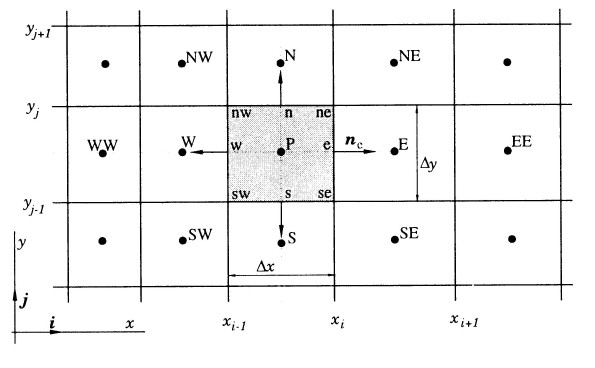
\includegraphics[scale=0.62]{3.jpg}\\
	\tiny{\underline{Source :} Cours Introduction à la Mécanique des Fluides Numériques : Méthode "Volumes Finis" - 1A HY - Alexeï Stoukov}
\end{frame}

\subsection[Simulation FF++]{Simulations avec FreeFem++}
\begin{frame}
	\frametitle{Résultats}
	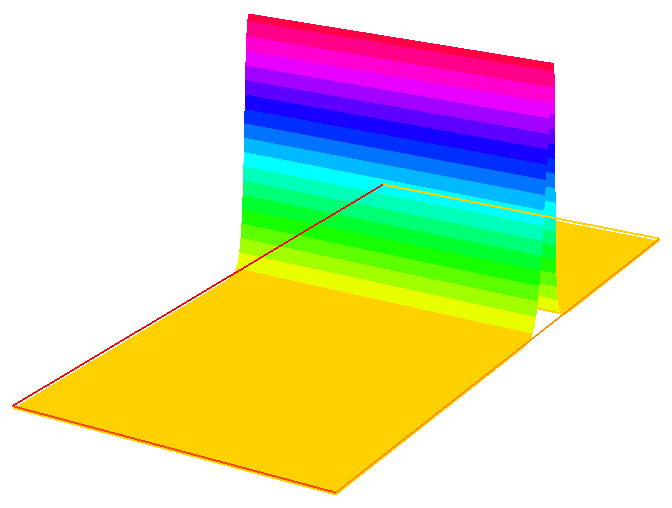
\includegraphics[scale=0.22]{../images/capture1.png}
	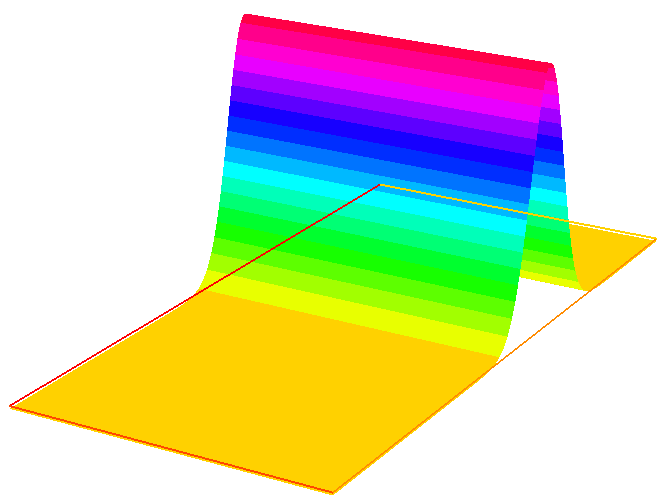
\includegraphics[scale=0.22]{../images/capture6.png}
	% Parler Sadaka, papier, etc. Essayer de faire pareil : merde encore. Parler aussi de FreeFem++
\end{frame}

\section*{Conclusion}
\begin{frame}
	\frametitle{Conclusion}
\end{frame}
\end{document}
